\documentclass[]{clearpath-user-manual}

\begin{document}

\thispagestyle{empty}
\begin{tikzpicture}[remember picture,overlay]
\node[anchor=north west,inner sep=0pt] at ($(current page.north west)+(0cm,0cm)$) {
  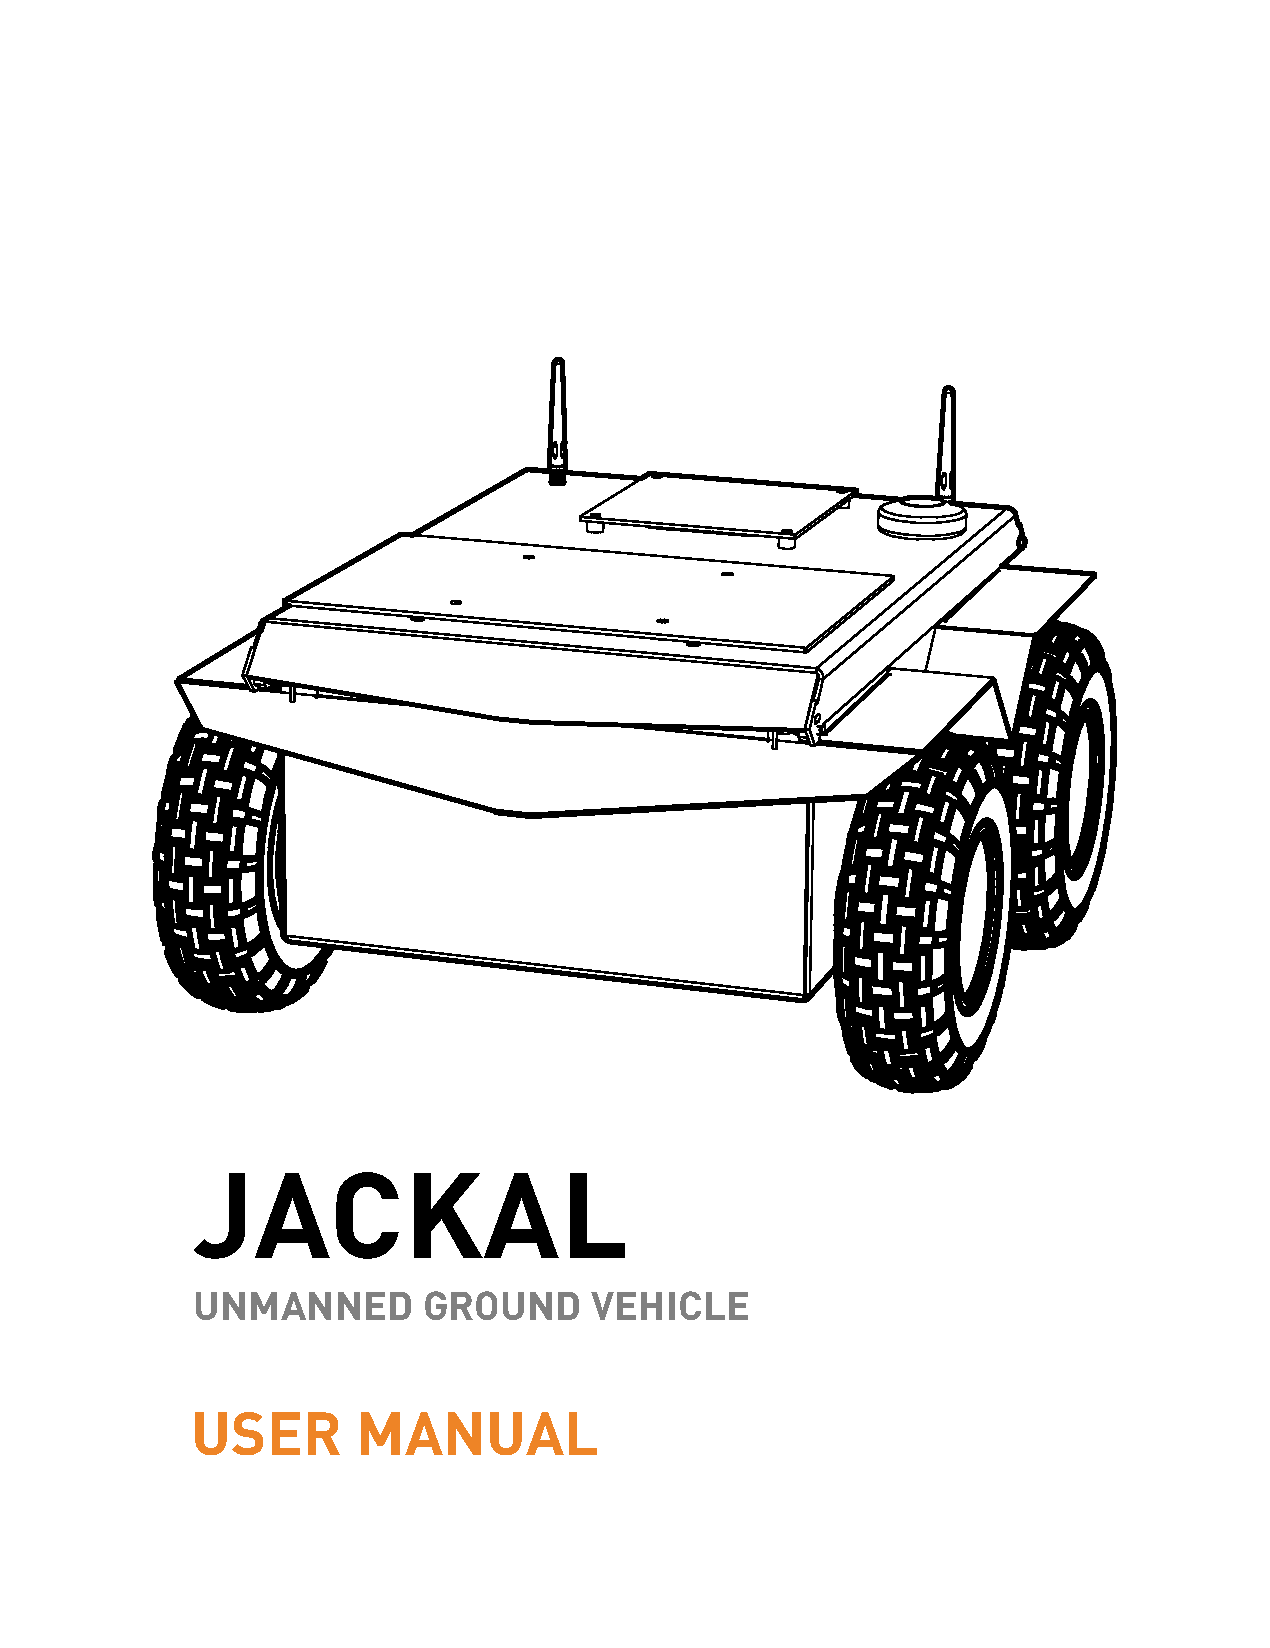
\includegraphics{gen/cover-page.pdf}
};
\end{tikzpicture}

\tableofcontents

\section{Introduction}

Jackal is a rugged, light, fast and easy-to-use unmanned ground vehicle for ROS Indigo, presented
by Clearpath Robotics.

Jackal includes a standard internal x86 PC, as well as basic IMU and GPS. Standard perception
modules are available, including URDF and simulator integration, and demonstration applications.
Please inquire with Clearpath Robotics for details.

\subsection{What's Included}

Contained in your Jackal shipment are the following items:

\begin{itemize}
  \item Jackal UGV
  \item 270 watt-hour lithium battery pack
  \item 110V/220V universal charger
  \item Sony Bluetooth controller
\end{itemize}

If you elected to purchase standard upgrade modules, these will be integrated into your Jackal chassis.

\section{Getting Started}

The first step is to power up your Jackal and have some fun driving it around!

\subsection{Talking to Jackal}

The next thing you probably want to do is get Jackal on your wireless network.

\subsection{Jackal Desktop}

To use Jackal from your desktop computer, first set up a basic ROS Installation. See the following
page for details:

\url{http://wiki.ros.org/indigo/Installation/Ubuntu}

When your ROS install is set up, install the Jackal desktop packages:

\begin{lstlisting}
sudo apt-get install ros-indigo-jackal-desktop
\end{lstlisting}

To connect to a running Jackal.


\end{document}
